\chapter{Semantics on the Fly} \label{chap:theory}
This chapter is concerned with a theoretical overview of a novel distributional semantic method designed to map words into conceptually productive geometric relationships.  At the heart of this approach is the idea that concepts, and, correspondingly, cognition are fundamentally contextual phenomena: by this view, concepts are process oriented, not objective, and so ``instantiating a concept is always a process of activating an ad hoc network of stored information in response to cues in context,'' \citep[][p. 546]{Casasanto2015}.  Language, as a mechanism for manipulating and transmitting cognitive content, is then likewise contextually situated, with meaning itself crucially being determined only in the moment of language use \citep{Evans2009}.  So, theoretically speaking, the method which will be described is based on some well travelled, if not entirely mainstream, ideas about the nature of language and mind:

\begin{enumerate}
\item{Concepts are not stable; they are generated in response to unfolding situations in an unpredictable environment;}
\item{Lexical semantics are accordingly always underspecified, and always resolved in some environmental context;}
\item{There is no relationship of strict supervenience between language and concepts one way or the other, but instead a dynamic by which concepts invite communication, and language affords conceptualisation.}
\end{enumerate}

These ideas, which have been outlined throughout the previous chapter, are not the standard dogma of computational linguistics, which generally, and understandably, has modelled concepts as modular, portable entities, language as a likewise stable system of representations and rules, and the relationship between the two as one of source and contingent data.  This structure-oriented approach to language and mind epitomises a project that \cite{Dreyfus2012} has described as ``finding the features, rules, and representations needed for turning rationalist philosophy into a research program,'' (p. 89).  As computer science and philosophy of mind increasingly interact at the vertex of cognitive modelling, culturally relative ideas about the connection between mental representations and linguistic symbols become incorporated into the very architecture of data structures, engendering a positive feedback loop by which the outputs of symbol manipulating information processing systems reinforce the premise that representations are stable entities which can be trafficked in the form of words according to the rules of a grammar.

I present the method outlined and tested in this thesis as an alternative to the foundationalist trend in computer science in general, and in computational linguistics in particular \citep[see][for a robust philosophical criticism of the idea that concepts are stable]{Rorty1979}.  This project involves trading the computational and mathematical allure of dimension reduction techniques and neural modelling, which have been prevalent in distributional semantic approaches, for a theoretically robust notion of situational context selection.  The methodology outlined theoretically in this chapter, and described technically in the next, has been conceived as a mechanism for the contextual generation of lexical representations that are structurally productive, in that the statistical features which make up a given representation define its geometric situation in relation to other representations in a particular context, and the geometry itself becomes semantically productive, with spatial relationships offering up interpretations of context specific word meanings.

I have no pretensions of instigating a paradigm shift in computer science.  I do not claim that the methodology I will now describe represents a radical departure from the prevailing and highly productive approach to the computational modelling of language or knowledge; indeed, it is very much grounded in the same broadly pragmatic considerations that have been the foundation of the statistical aspect of distributional semantics: word meaning is to an appreciable extent determined by the sentential context associated with observable word use.  My methodology is, rather, an attempt to build some consideration of the idea that minds are not populated by representations and that words are not static containers of meaning into the existing computational paradigm.  With this in mind, my model is predicated upon three interrelated desiderata, derived generally rather than in a one-for-one way from the points enumerated above:

\begin{enumerate}
\item The method should be dynamically sensitive to context;
\item The method should function in a way that is transparent and operationally interpretable;
\item The method should situate words in spaces which are likewise geometrically interpretable.
\end{enumerate}

The first stipulation encapsulates the theoretical premise of this work.  A primary objective of my methodology is to identify a statistically tangible mechanism for choosing word co-occurrence features in a contextually relevant way.  Specific mechanisms will be outlined in Chapter~\ref{chap:method}, and what counts as context will be discussed further in the course of the empirical results presented in Chapters~\ref{chap:similarity} and \ref{chap:figurative}, but the general idea is that a context sensitive model needs to react dynamically to information about what's happening in some linguistic situation.  The second requirement follows directly from the first: in order to pick semantic contexts \emph{in situ}, there needs to be a way to get a handle on the data which underwrites a model.  In practice this means that the scalars that form the basis for all the models which will be explored here represent literal information about co-occurrences in a large scale corpus, and the feature selections that take place in the course of delineating a contextual geometry can be traced to specific events in the underlying data.

Finally, the informationally transparent selection of contextual subspaces must result in a likewise interpretable geometry, where there is a coherent mapping between spatial features and semantic properties.  This last criterion in particular will lend the methodology one of its most powerful characteristics: by contextually selecting subspaces in which a variety of geometric relationships between word-vectors and more general features of the space can be analysed, we can hope to discover a single general way of representing a variety of semantic phenomena in a particular subspace.  As will be seen in Chapter~\ref{chap:method}, these subspaces will have a variety of geometric properties, including an origin, distance from an origin, and central and peripheral regions.  In this regard, my methodology presents an additional point of comparison with the standard distributional semantic approaches, which typically employ normalised spaces, often in the form of a hypersphere with both positive and negative values: while these are all vector space models and are all therefore to a certain extent concerned with extracting meaning from spatial relationships, my approach is in a certain respect \emph{more} geometrical, in that a variety of relationships, linear, angular, relative, and absolute, emerge in a given projection.  This geometric richness gives a model constructed using my methodology a wealth of interpretive features, ultimately allowing for the observation of different semantic properties -- for instance, similarity versus relatedness -- to emerge as different geometric aspects of the same subspace.

In the following three sections, each of these requirements will in turn be analysed in the context of the underlying theoretical context.  This analysis is performed with an eye towards the immediate project of designing a statistical model for mapping word-vectors to concepts by way of semantic geometry, and each element of the profile of desirable properties will be explored with this in mind.

\section{Dynamic Context Sensitivity}
At the heart of the technical work described in this thesis is an insight which is broadly accepted by theoretical linguists and philosophers of language: word meaning is always contextually specified.  This wisdom is built into the foundations of both formal semantics \citep{Montague1974} and pragmatics \citep{Grice1975}, and is likewise taken into account in contemporary context-free approaches to syntax \cite{Chomsky1986}.  As evident from the implementations of conceptual models surveyed in the previous chapter, however, the computational approach has generally relied on the idea that concepts can, at some level of composition, be cast as essentially static representations.  The tendency to treat concepts as self-contained ontological entities consisting of properties that are wholly or partly transferable is built into the fabric of the formal languages used to program computers, and indeed into the mechanisms of modular data processing systems with specific compartments for the storage and processing of data.\footnote{It is perhaps not a coincidence that Von Neumann was a seminal figure in the description of both the logic of lattice theory \citep{Birkhoff1958} that has motivated more recent developments in concept modelling such as formal concept analysis \citep{Wille1982} and the modular architecture of memory and processing components that defined computers in the period before the advent of highly parallel processing \citep{VonNeumann1945}.

With that said, the importance of context has certainly not been ignored by statistically oriented computer scientists.  Indeed, \cite{BaroniEA2014b} make a case for vector space approaches as a mechanism for ``disambiguation based on direct syntactic composition'' (p. 254), arguing that the linear algebraic procedures used to compose words into mathematically interpretable phrases and sentences in these types of models result in a systemic contextualisation of words in their pragmatic communicative context.  \cite{ErkEA2008} outlines an approach that models words as sets of vectors including prototypical lexical representations capturing information about co-occurrence statistics and ancillary vectors representing \emph{selectional preferences} \citep[\emph{per}][]{Wilks1978} gleaned from an analysis of the syntactic roles each word plays in its composition with other words.  These composite vector sets are then combined in order to consider the proper interpretation of multi-word constructs of lexically loose or ambiguous nouns and verbs.  In subsequent work, the same authors describe a model which selects \emph{exemplar} word-vectors from, again, composites of vectors, in this case extracted from observations of specific compositional instances of the words being modelled \citep{ErkEA2010}.  In the first instance, composition is the mechanism by which word meaning is selectively derived, while in the second instance observations of composition are the basis for constructing sets of representational candidates to be selected situationally.

The model presented in this thesis is motivated by a premise similar to the one explored by \citeauthor{ErkEA2008}: there should be some sort of selectional mechanism for choosing the way that a word relates to other words in context.  I would like to push this agenda a even further, though.  Following on \citepos{Barsalou} insight into the \emph{haphazard} way in which concepts emerge situationally, and likewise \citepos{Carston} proposition regarding \emph{ad hoc} conceptualisation, I propose that the mechanism for contextually mapping out conceptual relationships between representations of words should be as open ended as possible, ideally lending itself to the construction of novel conceptual relationships in the same way that the state space of possible word combinations offers an effectively infinite array of semantic possibilities.  In particular, I suggest that the ephemeral nature of concept formation can be modelled in terms of \emph{perspectives} on the conceptual affordances of lexical relationships.  Figure~\ref{fig:perspective} Illustrates this point.  From one point of view, \emph{dog} and \emph{cat} refer to exemplars of the conceptual category \textsc{pets}, while \emph{wolf} and \emph{lion} are typical of the category \textsc{predators}.  From a more taxonomically aligned point of view, though, \emph{dog} and \emph{wolf} group naturally in the \textsc{canine} category, while \emph{cat} and \emph{lion} clearly both belong to the category of \textsc{felines}.

\begin{figure}[t]
	\begin{subfigure}[t]{0.5\textwidth}
    \centering
	\begin{tikzpicture}[scale=0.07,baseline]
		\draw (0,0)--(-100,0)--(-100,-100)--(0,-100)--(0,0);
    	\draw (-15,-20) [left] node {wolf};
        \fill (-15,-20) circle[radius=1];
        \draw (-20,-75) [below] node {dog};
        \fill (-20,-75) circle[radius=1];
        \draw (-80,-80) [above] node {cat};
        \fill (-80,-80) circle[radius=1];
        \draw (-85,-25) [above] node {lion};
        \fill (-85,-25) circle[radius=1];
        \draw[fill=lightgray, fill opacity=0.25] (-17.5,-50) ellipse (10 and 48);
        \node at (-17.5,-50) {\LARGE canine};
        \draw[fill=lightgray, fill opacity=0.25] (-50,-77.5) ellipse (48 and 10);
        \node at (-50,-77.5) {\LARGE pet};
        \draw[fill=lightgray, fill opacity=0.25] (-82.5,-50) ellipse (10 and 48);
        \node at (-82.5,-50) {\LARGE feline};
        \draw[fill=lightgray, fill opacity=0.25] (-50,-22.5) ellipse (48 and 10);
        \node at (-50,-22.5) {\LARGE predator};
        \node at (-50,-102.5) [single arrow,draw,rotate=90,minimum height=40,minimum width=40,inner sep=15,opacity=0] {};
    \end{tikzpicture}
    \caption{a lexical space}
    \label{fig:bland}
    \end{subfigure}
    \begin{subfigure}[t]{0.5\textwidth}
    \centering
	\begin{tikzpicture}[scale=0.07,baseline]
    	\draw (0,0)--(-100,0)--(-100,-100)--(-57.5,-100);
        \draw (-42.5,-100)--(0,-100)--(0,-57.5);
        \draw (0,-42.5)--(0,0);
    	\draw (-15,-20) [above] node {wolf};
        \fill (-15,-20) circle[radius=1];
        \draw[dashed,->] (-15,-20)--(-15,-100);
        \draw (-15,-100) node {x};
        \draw[dashed,->] (-15,-20)--(0,-20);
        \draw (0,-20) node [rotate=90] {x};
        
        \draw (-20,-75) [above] node {dog};
        \fill (-20,-75) circle[radius=1];
        \draw [dashed,->] (-20,-75)--(-20,-100);
        \draw (-20,-100) node {x};
        \draw [dashed,->] (-20,-75)--(0,-75);
        \draw (0,-75) node [rotate=90] {x};
        
        \draw (-80,-80) [above] node {cat};
        \fill (-80,-80) circle[radius=1];
        \draw [dashed,->] (-80,-80)--(-80,-100);
        \draw (-80,-100) node {x};
        \draw [dashed,->] (-80,-80)--(0,-80);
        \draw (0,-80) node [rotate=90] {x};
        
        \draw (-85,-25) [above] node {lion};
        \fill (-85,-25) circle[radius=1];
        \draw [dashed,->] (-85,-25)--(-85,-100);
        \draw (-85,-100) node {x};
        \draw [dashed,->] (-85,-25)--(0,-25);
        \draw (0,-25) node [rotate=90] {x};
        
        \node at (3,-22.5) [below,rotate=90] {predator};
        \node at (3,-22.5) {\Large\}};
		
        \node at (3,-77.5) [below,rotate=90] {pet};
        \node at (3,-77.5) {\Large\}};
		
        \node at (-17.5,-103) [below] {canine};
        \node at (-17.5,-103) [rotate=-90] {\Large\}};

        \node at (-82.5,-103) [below] {feline};
        \node at (-82.5,-103) [rotate=-90] {\Large\}};
        
        \node at (-50,-102.5) [single arrow,draw,rotate=90,minimum height=40,minimum width=40,inner sep=15] {};
        \node at (-50,-102.5) {species};
        \node at (2.5,-50) [single arrow,draw,rotate=180,,minimum height=40,minimum width=40,inner sep=15] {};
        \node at (2.5,-50) {niche};
    \end{tikzpicture}
    \caption{a contextual projection}
    \label{fig:perspective}
    \end{subfigure}
  \caption{In the two-dimensional space depicted in (a), the conceptual vagary of four words maps to overlapping, elongated and indeterminate spaces.  In (b), two different perspectives on the lexical space, represented by the arrows labelled \emph{niche} and \emph{species}, offer contextualised projections in one-dimensional clusters which remit conceptual clarity.}
\end{figure}

Furthermore, the high dimensionality of vector space models of distributional semantics in particular should afford precisely these types of contextual vistas on potential relationships between words.  Rather than depending on \emph{a priori} disambiguation based on clustering or observations of context in the form of existing combinations of words, I propose that a technique for defining subspaces \emph{in situ} will capture the momentary and situated way in which concepts come about in the course of a cognitive agent's entanglement with the world.  The way that relationships between words coalesce and then dissolve as we change our perspective on the space of this model is designed to reflect the way that concepts emerge dynamically in the course of a cognitive agent's engagement with an environment.

This description of a process of perspective taking has thus far been quite high-level: that high dimensional spaces afford different vantage points on data is evident, but this begs the question of the actual mechanism for defining perspectives in such spaces.  The next section will focus on answering this question by outlining a method for 

\section{Literal Dimensions of Co-Occurrence}
The model presented here is grounded within the paradigm of distributional semantics, which means that the conceptual geometries that it constructs are the product of observations of word co-occurrences in a large-scale corpus of textual data represented statistically.  Two procedurally distinct methodological regimens have emerged from the recent study of distributional semantics.  The first, and more established, approach involves tabulating word co-occurrence frequencies and then using some function over these to build up word-vector representations.  With roots in the frequentist analysis described by \cite{SaltonEA1975}, recent research has typically involved matrix factorisation techniques presented as either (or both) an optimisation technique \citep{BullinariaEA2012} or a noise reducing mechanism \citep{KielaEA2014}.\footnote{\cite{BullinariaEA2012}, \cite{LapesaEA2013}, and \cite{KielaEA2014} have all reported that dimensional reduction techniques including SVD, random indexing, and top frequency feature selection generally do not improve results on word similarity and composition tests, with some notable parameter specific exceptions.}  A more recent approach, which has received a great deal of attention with the increasing availability of large-scale data and the corresponding advent of complex neural network architectures, involves using non-linear regression techniques to iteratively learn word-vector representations in an online, stepwise traversal of a corpus \citep{BengioEA2003,CollobertEA2008,KalchbrennerEA2014}.  \cite{BaroniEA2014} have described the former as \emph{counting} and the latter as \emph{predicting}, but it must be noted that both methods are very much grounded in observations about the co-occurrence characteristics of vocabulary words across large bodies of text.

Another important similarity between these two approaches is that they each in their own way move towards a representation of relationships between word-vectors which is to some extent optimally informative, and, by the same token, abstract.  In the instance of neural network approaches, this is clearly the case due to the fundamental nature of the system: the dimensions of this variety of model exist as basically arbitrary handles for gradually adjusting the relative positions of vectors, slightly altering every dimension of each vector each time the corresponding word is observed in the corpus.  And, as far as models based on explicit co-occurrence counts are concerned, the favoured technique tends to involve starting with a large, sparse space of raw co-occurrence statistics (frequencies, or, more typically, a mutual information type metric) and then factorising this matrix using a linear algebraic technique such as singular value decomposition.  The result, in either case, is a space of vectors which exists just for the sake of placing words in a relationship where distance corresponds to a semantic property, consisting of dimensions which can only be interpreted in terms of the way that they allow the model to relate words, not in terms of their relationship to the underlying data.  In fact, \cite{LevyEA2014b} have argued that recently developed neural networks approaches just exactly do recapitulate the process of matrix factorisation, and that a careful tuning of hyperparameters will generate commensurable results from either type of model.

A key feature of the model proposed in this thesis is that it maintains a space of highly sparse co-occurrence statistics, which, despite their anchoring in the relatively abstract realm of word positions in a digitised corpus, I will describe as \emph{literal} in the sense that they can be interpreted as corresponding to actual relationships between words in the world.  I don't wish to claim that there is scope for completely or even mainly recapitulating a nuanced conceptual model from the data available in a purely textual environment; to do so would be to move towards claims that intentionality can emerge from rule-based operations on symbols, and the problems with this have been explored by \citepos{Searle1980} Chinese room argument and a subsequent generation of philosophers \citep{PrestonEA2002}.  But I would like to suggest that by building a base model that maintains the accessibility of unreduced co-occurrence information, we likewise maintain the ability to manipulate this base model extemporaneously, in reaction to the ongoing emergence of new contextual information.  The idea is that such a base model would essentially represent the superset of all possible dimensions available for \emph{ad hoc} selection in the course of a 

So the proper framework for describing the model to be examined in this thesis is not so much a single space of word-vectors as a Grassmannian lattice consisting of the power set of all possible combinations of the dimensions characterising the base space.  At the top of this lattice -- the \emph{join} -- sits a single $k$-dimensional space consisting of every available one of the $k$ co-occurrence terms observed throughout the underlying corpus.  At the bottom of the lattice -- the \emph{meet} -- sit $k$ different one-dimensional spaces, each space corresponding to a single co-occurrence term.  If the meet is considered $layer-1$ of the lattice, and the join is considered layer $k$, then any given interstitial $layer-j$ consists of every possible combination of $j$ dimensions of co-occurrence statistics.  A diagram of a very simple example of one such model is presented in Figure~\ref{fig:lattice}, illustrating the possible subspaces projected from a vastly simplified model consisting of just three co-occurrence dimensions (these particular spaces will be explored in the next section, as illustrated in Figure~\ref{fig:instruments}.

\begin{figure}
\centering
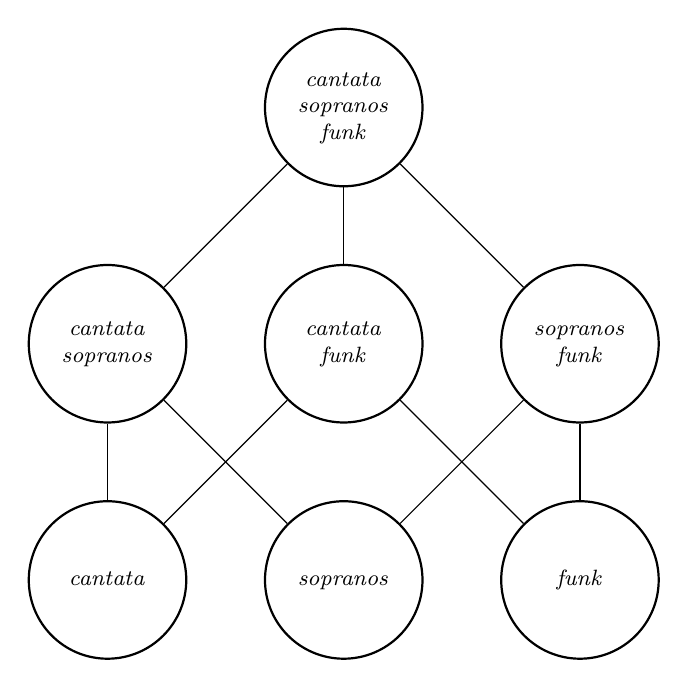
\begin{tikzpicture}[node distance=3cm,every node/.style={draw=black,thick,circle,inner sep=0pt}]
  \footnotesize
  \node[minimum size=2cm](join) {\begin{tabular}{c}
    \emph{cantata} \\
    \emph{sopranos} \\
    \emph{funk}
  \end{tabular}};
  \node[minimum size=2cm](two2) [below of=join] {\begin{tabular}{c}
    \emph{cantata} \\
    \emph{funk}
  \end{tabular}};
  \node[minimum size=2cm](two1) [left of=two2] {\begin{tabular}{c}
    \emph{cantata} \\
    \emph{sopranos}
  \end{tabular}};
    \node[minimum size=2cm](two3) [right of=two2] {\begin{tabular}{c}
    \emph{sopranos} \\
    \emph{funk}
  \end{tabular}};
  \node[minimum size=2cm](one2) [below of=two2] {\begin{tabular}{c}
    \emph{sopranos}
  \end{tabular}};
  \node[minimum size=2cm](one1) [left of=one2] {\begin{tabular}{c}
    \emph{cantata}
  \end{tabular}};
  \node[minimum size=2cm](one3) [right of=one2] {\begin{tabular}{c}
    \emph{funk}
  \end{tabular}};
  \draw (two1)--(join);
  \draw (two2)--(join);
  \draw (two3)--(join);
  \draw (one1)--(two1);
  \draw (one1)--(two2);
  \draw (one2)--(two1);
  \draw (one2)--(two3);
  \draw (one3)--(two2);
  \draw (one3)--(two3);
\end{tikzpicture}
\caption{A lattice of three dimensions, including the two-dimensional subspaces which are used for analysing the conceptual geometry of a small set of word-vectors in Figure~\ref{fig:instruments}}
\label{fig:lattice}
\end{figure}

An important distinction must be drawn, however, between the representation of my model as a lattice and the use of manifolds as an inferential mechanism.  Formal concept analysis in particular has made a productive discipline out of applying lattice type structures to conceptual modelling, using the semi-hierarchical properties of lattices to capture logical relationships of entailment \citep{Wille1982}.  That body of work takes as given that concepts are ``the basic units of thought formed in dynamic processes within social and cultural environments,'' \citep[][p. 2]{Wille2005}.  \cite{Widdows2004} offers a broad overview of how this approach might be pursued through corpus linguistic techniques, while \cite{GeffetEA2005} and, more recently, \cite{KartsaklisEA2016} have proposed statistical techniques using \emph{feature inclusion} metrics to assess the potential entailment relationship between candidate words and corresponding concepts.  The assumption inherent in this interesting work is that words are in some sense supervenient upon the concepts they denote, and that the statistical features of a language will by and large recapitulate the conceptual structure upon which it sits.

As \cite{Rimell2014} has pointed out, however, it is problematic to assume that a spectrum of co-occurrence alone can indicate relationships of hyponymy and hypernymy.  It stands to reason, for instance, that a word with a taxonomically specific referent such as \emph{bulldog} should probably have a co-occurrence profile including words omitted from the corresponding profile of a word like \emph{lifeform}, which has an ostensibly more general extent.  Rimell has proposed a measure of change in \emph{topic coherence} as word-vectors are combined algebraically in order to detect entailment relationships.  This measuring is achieved specifically through a process of dimension-by-dimensions comparison between potentially related word-vectors, in particular the \emph{vector negation} method described by \cite{Widdows2003}, combined with topic modelling techniques to analyse the coherence of features distilled by the selectional process.

The model proposed in this thesis adheres to the same principle of fine-grained cross-dimensional analysis described by Rimell.  In addition to the practical issues raised by Rimell, my model is also designed to remain pointedly uncommitted to any idea that concepts are atomic or elementary to thought, or that language and concepts are involved in any kind of strictly hierarchical relationships.  Instead, the model operates through an analytical traversal of a lattice of subspaces in search for a combination of dimensions that captures a conceptually \emph{salient} profile of co-occurrence features.  If a consequence of this stance is that the model can't be understood in terms of nested ordered relationships, though, then the question of how conceptual relationships do emerge situationally from the model remains.  The next section of this methodological overview will examine how the actual geometry of a projected subspace itself is expected to do this conceptual work.

\section{Interpretable Geometry}
It is important at this point to distinguish between two different modes of interpretability at play within the operation of the model I'm proposing.  On the one hand, we have the mechanism for selecting subspaces described above: this mechanism requires a model composed of tractable dimensions of statistics that can be interpreted based on expectations generated from an analysis of some sort of contextually relevant information.  Some specific mechanisms for this process will be discussed in the next section.  Then on the other hand, once this selectional process has taken place, we find ourselves with a subset of dimensions defining a specific subspace.  My claim is that, given the correct selectional criteria for performing this projection -- this traversal of our lattice of vector spaces -- we should be able to generate a subspace in which the projected word-vectors will be interpretable in terms of the actual geometric features of this subspace.

The idea of exploiting the geometry of a transformed space of word statistics is not new.  Indeed, seminal work on latent semantic analysis (LSA) was motivated by precisely the insight that a singular value decomposition of a high-dimensional, sparse matrix of statistical data about word co-occurrences would result in a dense lower dimensional matrix in which dimensions characterise \emph{latent semantics} rather than literal word co-occurrences \citep{DeerwesterEA1990}.  Thus the linear algebraic methodology of generating a lower dimensional matrix of optimally informative dimensions arguably transforms a space of specific co-occurrence events into a space of more general conceptual relationships.  In fact, \cite{LandauerEA1997} have subsequently argued that the dimensional reduction by way of factorisation itself might directly mirror cognitive conditioning, modelling the way that the mind can ``correctly infer indirect similarity relations only implicit in the temporal correlations of experience,'' (p. 212).

Of course the dimensions of a factorised matrix are still not interpretable in themselves.  They are, rather, an optimal abstraction of the underlying data, in which each dimension is maximally informative -- and, accordingly, orthogonal -- in comparison to the other dimensions.  What we desire in a model, however, is a mechanism for actually interpreting directions and regions within a subspace projected by the model.  This objective is motivated by \cite{Gardenfors2000} insight into the inferential power of \emph{conceptual spaces}: by building spaces in which the dimensions themselves correspond to \emph{properties}, G\"{a}rdenfors has illustrated how features of points and regions within these spaces such as convexity and betweeness can be interpreted as corresponding to conceptual membership and can accordingly be used to reason about relationships between concepts.  In more recent work, motivated by psycholinguist insight into the significance of the \emph{intersubjectivity} by which language facilitates the mutual ascription of cognitive content between interlocutors, \cite{Gardenfors2014} has proposed that semantics are derived from a communicative alignment of conceptual spaces.

A classic example of a G\"{a}rdenforsian conceptual space is the space of colors, which can be defined in terms of, for instance, hue, brightness, lightness, and colourfulness: any colour can be specified as a point corresponding to coordinates along each of these dimensions.  Moreover, regions within the space of colours can be defined geometrically: the concept \textsc{red} will correspond to a convex region within the space, and any point lying between two points known to be labelled \emph{red} will likewise be considered \emph{red}.  \cite{Jager} has devised an experiment mapping linguistic descriptions to conceptual regions precisely within the domain of colours.  Taking a large set of multi-lingual data regarding colour naming conventions, treating each of 330 different colours as an initially independent dimension, J\"{a}ger demonstrated how an extrapolation of optimally informational dimensions via a principle component analysis revealed clusterings of color names into convex regions.\footnote{The cross-cultural universality of colour naming conventions presented by \cite{KayEA1999}, which J\"{a}ger takes as a basis for his research, is controversial to say the least -- see \cite{Levinson2001} for an alternative point of view -- but J\"{a}ger's work remains a good example of a computational technique for extrapolating conceptual spaces from quantitative linguistic data.}

Similarly motivated by G\"{a}rdenfors's model of conceptual spaces, \cite{DerracEA2015} have built vectors of domain specific documents, associating word frequencies within documents with document labels.  A multi-dimensional scaling procedure is then used to project these document-vectors into a Euclidean space in which the authors predict that properties such as \emph{parallelness} and \emph{betweeness} will correspond to conceptual relationships between documents.  The authors demonstrate that geometry in their projected spaces does indeed afford conceptual interpretation: the word \emph{bog} is found to be more or less between \emph{heath} and \emph{wetland}, for instance, and the vector for the film \emph{Jurassic Park} lies in a direction associated with \textsc{dinosaurs} and \textsc{special effects}.  This work is particularly notable in that \citeauthor{DerracEA2015} appreciate the significance of projecting spaces which are interpretable in terms of Euclidean distances rather than simply the cosine similarity of vectors extending from the origin of a space: Euclidean metrics provide a platform for more nuanced considerations of the relationships between points.

The type of space exemplified by the research of J\"{a}ger and \citeauthor{Derrac} is moving towards being a conceptual space in the way that its geometry offers itself up to semantic interpretation, but importantly these remain static spaces comprised of abstract dimensions, albeit dimensions generated in order to optimise the interpretability of the spaces they delineate.  The objective of my model is to emulate the geometric interpretability of these other spaces in an extemporaneous, contextually dynamic way.  To illustrate this point, consider the two spaces illustrated in Figure~\ref{fig:instruments} (taken from real co-occurrence data, as described in the next section, and based on the lattice of subspaces illustrated in Figure~\ref{fig:lattice}).  Here co-occurrence statistics are used to define three different dimensions, from which two different two-dimensional subspaces are selected with word-vectors plotted into each subspace.  In each subspace, a particular conceptual geometry emerges, oblique to the axes of each subspace but nonetheless indicating distinct conceptual regions in which words cluster in an interpretable way.

\begin{figure}[t]
	\begin{subfigure}[t]{0.5\textwidth}
    \centering
	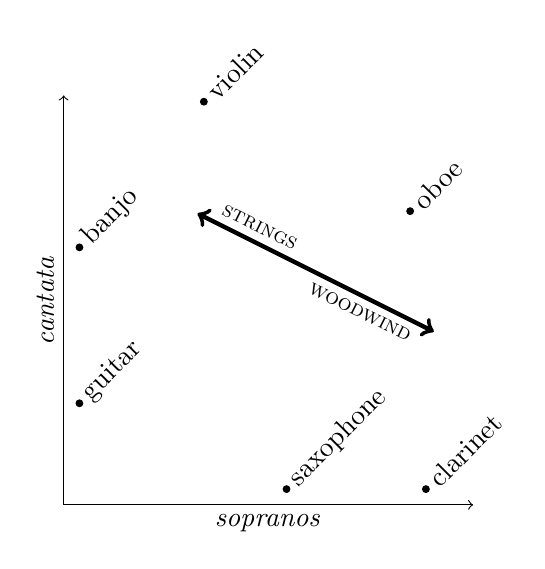
\begin{tikzpicture}[scale=1,baseline]
		\draw [->] (-0.2,-0.2)--(5,-0.2);
		\draw [->] (-0.2,-0.2)--(-0.2,5);
		\node at (2.4,-0.2) [below] {\emph{sopranos}};
		\node at (-0.2,2.4) [above,rotate=90] {\emph{cantata}};
		\draw [<->,ultra thick] (1.5,3.5)--(4.5,2);
		\node at (2.2,3.15) [above,rotate=-26.57] {\footnotesize \textsc{strings}};
		\node at (3.65,2.425) [below,rotate=-26.57] {\footnotesize \textsc{woodwind}};
		\node at (0.0,1.09) [right,rotate=45] {guitar};
		\fill (0.0,1.09) circle[radius=0.05];
		\node at (0.0,3.07) [right,rotate=45] {banjo};
		\fill (0.0,3.07) circle[radius=0.05];
		\node at (1.58,4.92) [right,rotate=45] {violin};
		\fill (1.58,4.92) circle[radius=0.05];
		\node at (2.63,0.0) [right,rotate=45] {saxophone};
		\fill (2.63,0.0) circle[radius=0.05];
		\node at (4.40,0.0) [right,rotate=45] {clarinet};
		\fill (4.40,0.0) circle[radius=0.05];
		\node at (4.20,3.53) [right,rotate=45] {oboe};
		\fill (4.20,3.53) circle[radius=0.05];
    \end{tikzpicture}
    \caption{\textsc{strings} vs \textsc{woodwind}}
    \label{fig:svsw}
    \end{subfigure}
    \begin{subfigure}[t]{0.5\textwidth}
    \centering
	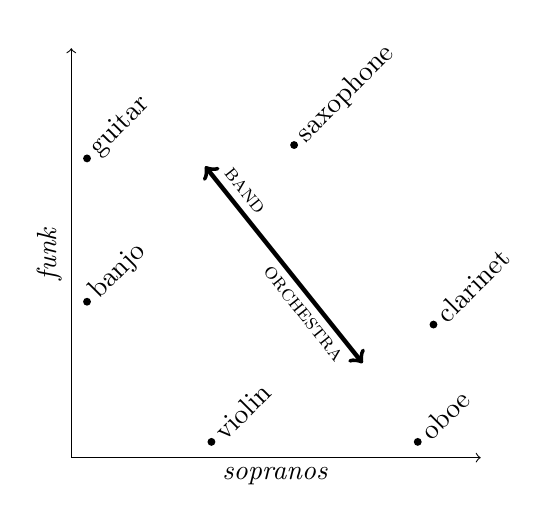
\begin{tikzpicture}[scale=1,baseline]
		\draw [->] (-0.2,-0.2)--(5,-0.2);
		\draw [->] (-0.2,-0.2)--(-0.2,5);
		\node at (2.4,-0.2) [below] {\emph{sopranos}};
		\node at (-0.2,2.4) [above,rotate=90] {\emph{funk}};
		\draw [<->,ultra thick] (1.5,3.5)--(3.5,1);
		\node at (1.85,3.0625) [above,rotate=-51.35] {\footnotesize \textsc{band}};
		\node at (2.9,1.75) [below,rotate=-51.35] {\footnotesize \textsc{orchestra}};
		\node at (0.0,3.60) [right,rotate=45] {guitar};
		\fill (0.0,3.60) circle[radius=0.05];
		\node at (0.0,1.78) [right,rotate=45] {banjo};
		\fill (0.0,1.78) circle[radius=0.05];
		\node at (1.58,0.0) [right,rotate=45] {violin};
		\fill (1.58,0.0) circle[radius=0.05];
		\node at (2.63,3.77) [right,rotate=45] {saxophone};
		\fill (2.63,3.77) circle[radius=0.05];
		\node at (4.40,1.49) [right,rotate=45] {clarinet};
		\fill (4.40,1.49) circle[radius=0.05];
		\node at (4.20,0.0) [right,rotate=45] {oboe};
		\fill (4.20,0.0) circle[radius=0.05];
    \end{tikzpicture}
    \caption{\textsc{band} vs \textsc{orchestra}}
    \label{fig:bvso}
    \end{subfigure}
  \caption{Based on real co-occurrence data, swapping one dimension in a two-dimensional subspace reveals two different conceptual geometries.}
  \label{fig:instruments}
\end{figure}

The first thing to note about these spaces is the way that swapping a single dimension in a two dimensional subspace can have a significant impact on the conceptual affordances of the subspace's geometry.  Realigning the relationships between terms along a single axis leads to a complete shift in the clusterings of terms, and, correspondingly, to the interpretation of regions and directions.  If these are conceptually sound subspaces, then we might expect word-vectors found within the area of the triangle described by the points labelled \emph{guitar}, \emph{banjo}, and \emph{violin} in Figure~\ref{fig:svsw} to be the names of other string instruments, or other conceptually relevant terms.  This is possibly asking too much of a subspace consisting of data regarding co-occurrences with just two terms across a large scale corpus, but as we scale up the dimensionality of the space -- as we ascend the lattice of subspaces of a fully realised model -- we can expect proper conceptual spaces to begin to coalesce.

The next thing to note is that the dimensions themselves are not especially interpretable.  While these dimensional profiles are explicable -- and indeed the ability to trace these statistics back to the corpus might turn out to be a desirable property for some applications -- the dimensions themselves do not conform to \citepos{Gardenfors2000} notion of dimensions as representing the properties that compose a concept.  It might be surprising, for instance, that the word \emph{cantata} has a higher propensity for co-occurrence with the word \emph{banjo} than with the word \emph{clarinet}, given that cantatas have traditionally included parts for the latter but not the former.  An examination of the underlying data, extracted, as described in the next section, from English language Wikipedia, reveals that the term \emph{cantata} has been adopted, perhaps somewhat figuratively, by some bluegrass musicians, and so co-occurrences with \emph{banjo} are indeed observed.

Rather than consider such usage as anomalous or attempt some sort of \emph{a priori} word sense disambiguation, I propose that we embrace the haphazardness of language and use it as a tool for projecting conceptually productive geometries.  In fact it would be surprising if it turned out that in anything other than the most specialised cases we could simply pick dimensions based on their labels and then expect co-occurrence statistics to play out in a conceptually coherent way, as this would contradict the Relevance Theoretic thesis that language in use is always significantly underspecified.  With this in mind, I suggest that we consider some set of dimensions, delineating a subspace and the corresponding geometry of word-vectors, to map precisely to a given context, and to effectively serve as the connective structure between language and conceptualisation.  Under this regimen, the dimensions themselves become the constitutive substance of a context, but they do not compositionally define any context in which they participate; rather, the contextualisation is an emergent property of the combination of dimensions underwriting it, corresponding to \emph{a way of speaking} about things.

The spaces illustrated in Figure~\ref{fig:instruments} are the product of a lattice consisting of combinations of just three dimensions, and as such the conceptual affordances of this toy model are highly limited.  As we add dimensionality to the model, however -- as we observe more terms co-occurring with our vocabulary of word-vectors -- we can expect an exponential growth in the combinatory possibilities of subspace construction.  With enough dimensions from which to choose, and with an appreciable degree of variance between the profiles of each dimensions, there should be scope for projecting more or less any constellation of word-vectors we desire.  The next question, then, is how to go about actually extracting a high dimensional base model of co-occurrence statistics from a large scale textual corpus.  The next section will answer this question.

%\section{A Computational Process}
%In this final section of this chapter, a technical implementation of the model described throughout the preceding three sections will be explained in detail.

%\subsection{A Large Scale Textual Corpus}
%The first step in a corpus based approach to natural language processing is the selection of the data which will provide the basis for our model.  I've picked the English language portion of Wikipedia as my data source, a choice which is in accordance with a good deal of work done in the field.  Some authors 

%In the case of the model used throughout this thesis, the November 2014 dump of English language Wikipedia has been used.\footnote{Accessible at XXX}  A data cleaning process has been implemented, the first step of which is the chunking of the corpus into individual sentences.  Next parenthetical phrases are removed from each sentence, as these can potentially skew co-occurrence data, and all other punctuation is subsequently removed.  All characters are converted into lowercase to avoid words capitalised at the beginning of sentences, quotations, and other places from being considered as unique types.  Finally, the articles \emph{a}, \emph{an}, and \emph{the} are removed as they can distort co-occurrence windows (consider, for instance, how these terms affect the proximity of the other words in the phrase ``a mouse, an owl, and a dog sat on the moon'').  The cleaned corpus contains about

%-WORD, SENTENCE COUNTS

%As is generally the case with data cleaning, these measures are prone to error: for instance, due to the removal of punctuation, the contraction \emph{we're} will be considered identical to the word \emph{were}.  One of the strengths of the subspace projection technique that my model uses is its resilience to noise.  So, for instance, misspellings will be categorised as highly anomalous co-occurrence dimensions and are therefore unlikely to be contextually selected -- or, if they are regularly encountered enough to be contextually significant, there may well be useful information in the co-occurrence profile of such mistakes -- and essentially ubiquitous words are unlikely to provide context specific information, so the ambiguity between \emph{we're} and \emph{were} is unlikely to be drawn into any of the subspaces actually projected by the model.

%From the cleaned corpus, the model's vocabulary is defined as the top 200,000 most frequently occurring word types.  This cut-off point is very close to the point where the total number of word tokens included -- that is, occurrences of any word of any type -- included by selecting all instances of all vocabulary words equals the total number of word types -- that is, unique word forms -- excluded.  Given the Zipfian distribution of word frequencies as observed throughout the corpus, this means that more than 95\% of the co-occurrence data available from the corpus will be taken into account by the model, while the number of word-vectors used to express this data represents less than 5\% of the potential vocabulary---a fairly efficient way of extrapolating statistics from the corpus.

%- human vocabulary size

%\subsection{Mutual Information of Word Co-Occurrences}
%The critical event in the 

%Here, following the example of almost all distributional semantic work, co-occurrence between a word $w$ and another word $c$ will be considered in terms of the number of other words between $w$ and $c$.  In the case of my model, again in accord with the a great deal of work within the field, a statistic for word $w$ in terms of its co-occurrence with $c$ will be derived from the consideration of all the times that $c$ is observed within $k$ words of $w$, where $k$ is one of the primary model parameters that will be considered in the experiments reported in later chapters of this thesis.  Based on these co-occurrence events, a matrix $M$ is defined, where rows consist of word-vectors, one for each of the 200,000 words in the vocabulary, and columns correspond to terms with which these vocabulary words co-occur.  These column-wise co-occurrence dimensions include the words in the vocabulary, including the possible co-occurrence of a word with itself (``a \emph{rose} is a \emph{rose} is a \emph{rose}'', for instance) as well as many, many words that are not in the vocabulary, to the extent that every word type in the corpus is considered as a dimension of co-occurrence.

%In this last respect, my model diverges from the typical approach, which usually seeks to limit not only the vocabulary but also the dimensionality of the underlying co-occurrence matrix.  This has typically involved a curtailing of the number of co-occurrence terms at both ends of the frequency spectrum, based on the assumption that both high frequency so-called function words (the prepositions, conjunctions, and so forth) and low frequency terms such as obscure proper names will muddy a model with either general flattening or highly topical skewing.  In the case of my model, however, these problems are irrelevant, as dimensions will be selected on a case-by-case, context specific basis, and there is no good reason to discard information which may in some possibly unforeseen circumstance prove relevant.  The result is a 200,00 by $\approx$ 7.5 million matrix $M$ where a scalar corresponding to co-occurrences between $w$ and $c$ is defined in terms of this equation:

%\begin{equation}\label{eq:MI}
%M_{w,c} = \log_2 \left(\frac{n_{w,c} \times W}{n_w \times \left(n_c + a\right)} + 1\right)
%\end{equation}

%Here $n_{w,c}$ represents the total number of times that that $c$ is observed as co-occurring in a sentence within $k$ words on either side of $w$, $n_w$ is the independent frequency of occurrences of $w$, and $c$ is likewise the overall frequency of $c$ being observed as a co-occurrence term throughout the corpus.  $W$ is the overall occurrence of all words throughout the corpus---and it should be noted that, excluding the term $a$, the ratio in Equation~\ref{eq:MI} is equivalent to the joint probability of $w$ and $c$ co-occurring.  The application of a logarithm to this ratio, again a common practice, is in the spirit of \citepos{Shannon} information theory, and is 

%The term $a$ is a skewing constant used to prevent highly specific co-occurrences from dominating the analysis of a word's profile, set for the purposes of the work reported here at 10,000.\footnote{Anecdotally, the first combination of input words analysed during an early stage of the development of this model that didn't use a smoothing constant was the phrase ``musical creativity'', and the very first dimension indicated by the analysis was labelled \emph{gwiggins}---my primary supervisor's email handle.  Prof. Wiggins's deep connection with music and creativity meant that every instance of \emph{gwiggins} occurring throughout Wikipedia was in the vicinity of both \emph{musical} and \emph{creativity}, and so the dimension was indicated by the combination of these terms, which makes sense, but it was still a bit eerie to have such a personally relevant result generated by a model based on such general data.}

%Finally, the entire ratio is skewed by 1 so that all values returned by the logarithm will be greater than 0, with a value of zero therefore indicating that two words have never been observed to co-occur with one another.  This is again a departure from standard practice, where, in word counting models, a \emph{pointwise mutual information} mechanism involving not skewing the ratio and instead treating any ratio of frequencies less than 1 -- that is, any co-occurrence that is observed less than often than balance of the mean values for all occurrences of $w$ and all co-occurrences with $c$ -- as being equivalent to 0, or no co-occurrence at all.  The motivation for this more typical technique is again to avoid incorporating unnecessary and potentially confounding information into a model, but, again, in the case of my model, the dimensional selection process will tend to ignore such information, and at the same time, as will be seen, data regarding relatively unlikely co-occurrences can sometimes also be quite informative.  In support of my technique, it is worth mentioning that the vast majority of potential co-occurrences will never be observed, and, at the same time, a comprehensive language model should maintain at least the possibility of any co-occurrence

%\cite{Brown}

%so there seems to be wisdom in the idea of not throwing away information about even relatively unlikely linguistic events.

%\subsection{Dimensional Selection Techniques}
%Having established a base model of co-occurrence statistics, the 

%\begin{equation}\label{eq:oldNorm}
%w^j_i = \frac{w^j_i}{\sqrt{\sum_{k=1}^{b} \left(w^k_i\right)^2}}
%\end{equation}

%\begin{equation}\label{eq:Norm}
%w^j_i = \frac{w^j_i}{\sum_{k=1}^{b} abs\left(w^k_i\right)}
%\end{equation}

%\begin{equation}\label{eq:Arg}
%\mu_c =  \frac{1}{n} \sum_{w=1}^{n}N_{w,c}
%\end{equation}

%\begin{equation}\label{eq:Trans}
%M_{w,c} \Rightarrow S_{w,c'}
%\end{equation}
%\subsection{Extracting Semantics from Geometric Features}
